% Provenance (never printed): see sources/outline_sources.md (Year 1: internal
% structure of the Earth from seismology; reference model; density, gravity and
% pressure inside the Earth; mantle mineralogy; lithosphere and asthenosphere).
% Curves from figdata/bachelor-1/prem_profiles.py (shared dataset data:prem) and
% figdata/bachelor-1/refraction.py (generic two-layer crust); exercise and problem
% values in the Book 3 scratch calculator calc/ch09.py.
\chapter{La Terre en couches}\label{ch:b1:layered-earth}

Le 8 octobre 1909, un séisme ébranla la vallée de la Kupa, au sud-est de Zagreb.
% ledger: skoko:mohorovicic
Andrija Mohorovičić, qui dirigeait l'observatoire de la ville, rassembla les
sismogrammes enregistrés à travers l'Europe et remarqua quelque chose d'étrange~:
jusqu'à quelques centaines de kilomètres de l'épicentre, la première secousse
arrivait d'une façon, plus loin un second type de première arrivée prenait le
relais, comme si une part de l'énergie avait trouvé une voie plus rapide en
profondeur. Il l'expliqua par une limite située à quelque cinquante kilomètres de
profondeur, au-dessous de laquelle les ondes vont plus vite~: la base de la
\omterm{def:b1:layered-earth:layers}{croûte}. Un siècle de tels enregistrements, des millions, a fait de cette première
limite un modèle de référence de la Terre entière, couche par couche, avec ses
vitesses, sa masse volumique, sa pesanteur et sa pression jusqu'au centre. Ce
chapitre montre comment on trouve une limite à partir des temps de trajet, ce que
dit le modèle de référence, comment on dessine un profil de masse volumique à
partir des seules vitesses sismiques et on le vérifie avec la masse et le moment
d'inertie de la Terre, quels minéraux constituent le \omterm{def:b1:layered-earth:layers}{manteau} à chaque profondeur,
de quoi est fait le noyau, et où s'arrête l'enveloppe rigide externe de la
planète.

\begin{recall}
Une onde P est une onde de compression, une onde S une onde de cisaillement~; les
ondes S ne traversent pas les liquides, et les zones d'ombre des ondes P et S du
noyau donnent le rayon du \omterm{def:b1:layered-earth:layers}{noyau externe} liquide (livre~2, année~11). Les ondes
sont réfractées à une limite selon la loi de Snell--Descartes,
$\sin i_1/v_1 = \sin i_2/v_2$ (physique). Dans un fluide au repos, la pression
croît avec la profondeur comme $\mathrm dP = \rho g\,\mathrm dz$ (physique, volume
de première année). La \omterm{def:b1:layered-earth:layers}{croûte}, le \omterm{def:b1:layered-earth:layers}{manteau} et le noyau ont été introduits au
livre~1 (année~6).
\end{recall}

\section{Les ondes sismiques dans une Terre en couches}

Les vitesses des ondes sismiques dépendent des modules d'élasticité de la roche et
de sa masse volumique. Les livres de physique les déduisent des équations de
l'élasticité des milieux continus~; elles sont ici supposées connues.

\begin{proposition}[Vitesses sismiques]\label{prop:b1:layered-earth:speeds}
Dans un solide élastique isotrope de masse volumique $\rho$, de module
d'incompressibilité $K$ et de module de cisaillement $\mu$, les ondes P et S se
propagent à
\[
  v_P = \sqrt{\frac{K + \tfrac43\mu}{\rho}}, \qquad v_S = \sqrt{\frac{\mu}{\rho}}.
\]
Dans un liquide $\mu = 0$~: $v_S = 0$ et aucune onde S ne se propage.
\end{proposition}
\admitted

Comme $K$ et $\mu$ sont positifs, $v_P > v_S$ toujours~: dans la \omterm{def:b1:layered-earth:layers}{croûte} et le
\omterm{def:b1:layered-earth:layers}{manteau} de PREM, $v_P$ vaut environ $1.8$ à $1.9$ fois $v_S$, et les ondes P
arrivent en premier. Les deux vitesses croissent en général avec la profondeur,
parce que la pression rigidifie la roche plus qu'elle ne la comprime, si bien que
les rayons s'incurvent vers la surface~; et à quelques profondeurs elles sautent.

\begin{definition}[Discontinuité sismique, Moho, limites noyau--manteau et du noyau interne]
\label{def:b1:layered-earth:discontinuity}
Une \emph{discontinuité sismique}\index{discontinuite sismique@discontinuité sismique} est une surface à l'intérieur de la Terre à travers
laquelle les vitesses sismiques, la masse volumique ou les deux changent
brusquement, sur une épaisseur petite devant une longueur d'onde sismique. La
\emph{discontinuité de Mohorovičić}\index{discontinuite de Mohorovicic@discontinuité de Mohorovičić} (ou
\emph{Moho}\index{Moho}) est la base de la \omterm{def:b1:layered-earth:layers}{croûte}, où $v_P$ saute à environ
\qty{8}{km.s^{-1}}. La \emph{limite noyau--manteau}\index{limite noyau--manteau} est la surface entre le \omterm{def:b1:layered-earth:layers}{manteau}
silicaté solide et le \omterm{def:b1:layered-earth:layers}{noyau externe} liquide~; la \emph{limite du noyau
interne}\index{limite du noyau interne} est la surface entre le \omterm{def:b1:layered-earth:layers}{noyau externe} liquide et le \omterm{def:b1:layered-earth:layers}{noyau interne}
solide.
\end{definition}

\subsection{Réfraction à la limite d'une couche}

Prenons une couche d'épaisseur $h$ et de vitesse $v_1$, la \omterm{def:b1:layered-earth:layers}{croûte}, au-dessus d'un
demi-espace de vitesse $v_2 > v_1$, le \omterm{def:b1:layered-earth:layers}{manteau}, et une source à la surface. Trois
ondes parviennent à un récepteur à la distance $x$. L'onde directe se propage dans
la couche, à $v_1$. L'onde réfléchie rebondit sur la limite. Et un rayon qui
frappe la limite à l'angle critique $i_c$, avec $\sin i_c = v_1/v_2$, est
réfracté le long d'elle, se propage dans le milieu plus rapide juste au-dessous à
la vitesse $v_2$, et renvoie de l'énergie vers le haut dans la couche sous le même
angle $i_c$ tout le long de son trajet.

\begin{definition}[Onde conique, distance de croisement]\label{def:b1:layered-earth:head-wave}
Une \emph{onde conique}\index{onde conique} est l'onde qui se propage le long d'une limite à la
vitesse du milieu le plus rapide situé au-dessous et la quitte vers le haut sous
l'angle critique. La \emph{distance de croisement}\index{distance de croisement} est la distance à la source au-delà
de laquelle l'onde conique arrive avant l'onde directe.
\end{definition}

\begin{theorem}[Temps de trajet au-dessus d'une Terre à deux couches]\label{thm:b1:layered-earth:two-layer}
Au-dessus d'une couche d'épaisseur $h$ et de vitesse $v_1$ reposant sur un
demi-espace de vitesse $v_2 > v_1$, une source en surface et un récepteur en
surface à la distance $x$ donnent
\[
  t_{\text{direct}} = \frac{x}{v_1}, \qquad
  t_{\text{conique}} = \frac{x}{v_2} + \frac{2h\cos i_c}{v_1}
  \quad (x \ge 2h\tan i_c), \qquad \sin i_c = \frac{v_1}{v_2},
\]
et l'\omterm{def:b1:layered-earth:head-wave}{onde conique} arrive la première au-delà de la \omterm{def:b1:layered-earth:head-wave}{distance de croisement}
\[
  x_c = 2h\sqrt{\frac{v_2 + v_1}{v_2 - v_1}}.
\]
\end{theorem}

\begin{proof}
L'\omterm{def:b1:layered-earth:head-wave}{onde conique} descend sous l'angle $i_c$ à travers la couche, sur un trajet de
longueur $h/\cos i_c$, court le long de la limite sur la distance
$x - 2h\tan i_c$, et remonte sur un trajet de longueur $h/\cos i_c$. Son temps de
trajet est
\[
  t_{\text{conique}} = \frac{2h}{v_1\cos i_c} + \frac{x - 2h\tan i_c}{v_2}
  = \frac{x}{v_2} + \frac{2h}{v_1\cos i_c}\Bigl(1 - \frac{v_1\sin i_c}{v_2}\Bigr)
  = \frac{x}{v_2} + \frac{2h}{v_1\cos i_c}\,(1 - \sin^2 i_c),
\]
c'est-à-dire $x/v_2 + 2h\cos i_c/v_1$. Le trajet n'existe que si le parcours
horizontal est positif, $x \ge 2h\tan i_c$. Les deux temps sont égaux lorsque
$x(1/v_1 - 1/v_2) = 2h\cos i_c/v_1$~; avec $\cos i_c = \sqrt{v_2^2 - v_1^2}/v_2$,
\[
  x\,\frac{v_2 - v_1}{v_1 v_2} = \frac{2h\sqrt{(v_2 - v_1)(v_2 + v_1)}}{v_1 v_2},
\]
ce qui donne $x_c$. Au-delà, la droite de l'\omterm{def:b1:layered-earth:head-wave}{onde conique}, de plus petite pente
$1/v_2$, passe sous la droite de l'onde directe.
\end{proof}

Sur un graphique du temps de trajet en fonction de la distance, les ondes directe
et conique sont deux droites. Leurs pentes sont les inverses des vitesses $1/v_1$
et $1/v_2$~; la droite de l'\omterm{def:b1:layered-earth:head-wave}{onde conique}, prolongée jusqu'à $x = 0$, coupe l'axe
des temps au \emph{temps d'interception} $t_i = 2h\cos i_c/v_1$. L'onde réfléchie,
$t = \sqrt{x^2 + 4h^2}/v_1$, est une hyperbole qui touche la droite de l'\omterm{def:b1:layered-earth:head-wave}{onde
conique} à la distance critique $2h\tan i_c$, où naît l'\omterm{def:b1:layered-earth:head-wave}{onde conique}
(\cref{exo:b1:layered-earth:10}).

\begin{omfigure}
\begin{tabular}{@{}c@{}}
\begin{tikzpicture}
\begin{axis}[width=0.86\linewidth, axis equal image, xmin=0, xmax=260, ymin=-62, ymax=8,
  axis x line=top, axis y line=left, axis line style={-}, clip=false,
  ylabel={profondeur (km)}, ytick={-60,-35,0},
  yticklabels={60,35,0}, tick label style={font=\scriptsize}, label style={font=\small}]
\fill[brown!12] (axis cs:0,0) rectangle (axis cs:260,-35);
\fill[orange!18] (axis cs:0,-35) rectangle (axis cs:260,-62);
\draw[black!60] (axis cs:0,-35) -- (axis cs:260,-35);
\addplot[very thick, blue!70!black] table[x=x, y=z, unbounded coords=jump,
  restrict expr to domain={\coordindex}{0:1}] {figdata/out/bachelor-1-refraction-rays.dat};
\addplot[thick, dashed, green!45!black] table[x=x, y=z, unbounded coords=jump,
  restrict expr to domain={\coordindex}{3:5}] {figdata/out/bachelor-1-refraction-rays.dat};
\addplot[very thick, red!75!black] table[x=x, y=z, unbounded coords=jump,
  restrict expr to domain={\coordindex}{7:10}] {figdata/out/bachelor-1-refraction-rays.dat};
\node[font=\scriptsize, anchor=north west] at (axis cs:2,-36) {manteau, $v_2 = \qty{8.0}{km.s^{-1}}$};
\node[font=\scriptsize, anchor=center] at (axis cs:125,-17) {croûte, $v_1 = \qty{6.0}{km.s^{-1}}$, $h = \qty{35}{km}$};
\node[font=\scriptsize, red!75!black, anchor=north] at (axis cs:150,-36) {onde conique le long du Moho};
\node[font=\scriptsize, green!45!black, anchor=south] at (axis cs:40,-20) {réfléchie};
\node[font=\scriptsize, blue!70!black, anchor=north] at (axis cs:125,-1) {directe};
\fill (axis cs:0,0) circle (2pt);
\end{axis}
\end{tikzpicture}\\[2pt]
{\small (a) trajets des rayons (distance en km)}\\[6pt]
\begin{tikzpicture}
\begin{axis}[omrecord, width=0.86\linewidth, height=6.0cm, xmin=0, xmax=400, ymin=0, ymax=70,
  xlabel={distance $x$ (km)}, ylabel={temps de trajet $t$ (s)}, tick label style={font=\scriptsize},
  label style={font=\small}, clip=false,
  legend style={font=\scriptsize, at={(0.03,0.97)}, anchor=north west, draw=none, fill=white, fill opacity=0.85}]
\addplot[very thick, blue!70!black] table[x=x, y=t_direct] {figdata/out/bachelor-1-refraction-times.dat};
\addlegendentry{directe, pente $1/v_1$}
\addplot[thick, dashed, green!45!black] table[x=x, y=t_reflected] {figdata/out/bachelor-1-refraction-times.dat};
\addlegendentry{réfléchie}
\addplot[very thick, red!75!black, unbounded coords=jump] table[x=x, y=t_head] {figdata/out/bachelor-1-refraction-times.dat};
\addlegendentry{onde conique, pente $1/v_2$}
\addplot[thin, dotted, red!75!black, domain=0:79.37] {x/8 + 7.717};
\draw[black!60, densely dashed] (axis cs:185.2,0) -- (axis cs:185.2,30.87);
\node[font=\scriptsize, anchor=north west] at (axis cs:187,8) {$x_c = \qty{185}{km}$};
\node[font=\scriptsize, anchor=east, red!75!black] at (axis cs:-3,7.7) {$t_i$};
\end{axis}
\end{tikzpicture}\\[2pt]
{\small (b) temps de trajet}
\end{tabular}

\par\smallskip{\small Réfraction au-dessus d'une \omterm{def:b1:layered-earth:layers}{croûte} de \qty{35}{km}
d'épaisseur, à \qty{6.0}{km.s^{-1}}, sur un \omterm{def:b1:layered-earth:layers}{manteau} à \qty{8.0}{km.s^{-1}} ((a) à
l'échelle vraie). (a) L'onde directe court le long de la surface~; l'onde
réfléchie dessinée est celle qui frappe le \omterm{def:b1:layered-earth:discontinuity}{Moho} à l'angle critique,
\ang{48.6}~; l'\omterm{def:b1:layered-earth:head-wave}{onde conique} court le long du \omterm{def:b1:layered-earth:discontinuity}{Moho} et revient sous cet angle. (b)
Temps d'arrivée~: l'\omterm{def:b1:layered-earth:head-wave}{onde conique} apparaît à la distance critique,
\qty{79}{km}, tangente à la réflexion, et dépasse l'onde directe à la \omterm{def:b1:layered-earth:head-wave}{distance de
croisement}, \qty{185}{km}. Le prolongement en pointillés donne le temps
d'interception $t_i = \qty{7.7}{s}$.}
\end{omfigure}

\begin{method}[La profondeur d'une limite d'après un profil de réfraction]\label{met:b1:layered-earth:moho}
\begin{enumerate}
  \item Tracer les temps de première arrivée en fonction de la distance, et
        ajuster une droite sur les arrivées proches de la source et une autre sur
        les arrivées lointaines.
  \item Les pentes inverses donnent $v_1$ et $v_2$~; alors $\sin i_c = v_1/v_2$.
  \item Lire le temps d'interception $t_i$ de la droite lointaine en $x = 0$, et
        calculer $h = t_i v_1/(2\cos i_c)$~; le vérifier avec la \omterm{def:b1:layered-earth:head-wave}{distance de
        croisement}, $h = \tfrac12 x_c\sqrt{(v_2 - v_1)/(v_2 + v_1)}$.
  \item Une limite n'est trouvée que si $v_2 > v_1$~: une couche plus lente sous
        une couche plus rapide ne produit pas d'\omterm{def:b1:layered-earth:head-wave}{onde conique} et reste cachée.
\end{enumerate}
\end{method}

Les deux sortes de première arrivée de Mohorovičić étaient exactement ces deux
droites~: l'onde directe dans la \omterm{def:b1:layered-earth:layers}{croûte} près de la source, l'\omterm{def:b1:layered-earth:head-wave}{onde conique} le long
du toit du \omterm{def:b1:layered-earth:layers}{manteau} plus loin. Son chiffre pour l'épaisseur de la \omterm{def:b1:layered-earth:layers}{croûte} dans cette
région, \qty{54}{km}, a été confirmé dans son ordre de grandeur, mais la
profondeur du \omterm{def:b1:layered-earth:discontinuity}{Moho} varie d'un endroit à l'autre. Sous les océans, la \omterm{def:b1:layered-earth:layers}{croûte} n'a
qu'environ \qty{5}{km} d'épaisseur~; sous les continents, elle en a en moyenne
environ \qty{30}{km}, et elle est bien plus épaisse sous les grandes chaînes de
montagnes. Pour son modèle de référence, PREM a placé le \omterm{def:b1:layered-earth:discontinuity}{Moho} à \qty{11}{km} sous
le niveau de la mer sous les océans et à \qty{35}{km} sous les continents.
% ledger: skoko:mohorovicic, usgs:crust-thickness, prem:moho-average

\begin{history}[Andrija Mohorovičić]
\begin{minipage}[t]{0.76\linewidth}\vspace{0pt}
% ledger: skoko:mohorovicic
Andrija Mohorovičić (1857--1936) vint à la sismologie par la météorologie~:
enseignant, puis de 1891 à 1921 directeur de l'observatoire météorologique de
Zagreb, il publia sa dernière étude météorologique en 1901. Sur les sismogrammes
du séisme de la vallée de la Kupa du 8 octobre 1909, il trouva deux paires
distinctes de phases P et S~: près de la source un type de première secousse
arrivait en premier, plus loin un autre, qui avait voyagé plus vite en profondeur.
Sa lecture de ces deux arrivées comme une onde directe et une onde réfractée
sous une limite donna la limite qui porte aujourd'hui son nom, et la première
mesure de l'épaisseur de la \omterm{def:b1:layered-earth:layers}{croûte}.
\end{minipage}\hfill
\begin{minipage}[t]{0.2\linewidth}\vspace{0pt}
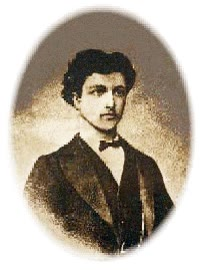
\includegraphics[width=\linewidth]{images/book3/b1-mohorovicic.jpg}

{\scriptsize Andrija Mohorovičić. Domaine public.}
\end{minipage}
\end{history}

\section{Un modèle de Terre de référence}

Le même raisonnement, appliqué à des millions de temps de trajet à toutes les
distances et aux périodes des oscillations libres de la Terre (la planète entière
résonne comme une cloche après un grand séisme), donne les vitesses à chaque
profondeur.

\begin{definition}[Modèle de Terre de référence]\label{def:b1:layered-earth:reference-model}
Un \emph{modèle de Terre de référence}\index{modele de Terre de reference@modèle de Terre de référence} est une Terre à symétrie sphérique, donnée par
les vitesses sismiques $v_P(r)$, $v_S(r)$, la masse volumique $\rho(r)$ et, dans
les modèles les plus complets, l'atténuation, comme fonctions du seul rayon $r$,
qui s'accorde avec les temps de trajet observés, les périodes d'oscillations
libres, la masse de la Terre et son moment d'inertie. Le plus employé est PREM, le
modèle de Terre de référence préliminaire (1981).
\end{definition}

PREM a été ajusté au rayon \qty{6371}{km}, à la masse
\qty{5.974e24}{kg} et au \omterm{def:b1:comparative-planetology:moi}{facteur de moment d'inertie} $0.3308$ de la Terre.
Il divise la planète en quelques régions jointes par des discontinuités, et ses
profils (figure ci-dessous) montrent d'emblée les couches principales.

\begin{definition}[Croûte, manteau, noyau externe, noyau interne]\label{def:b1:layered-earth:layers}
La \emph{croûte}\index{croute@croûte} est la couche silicatée externe au-dessus du \omterm{def:b1:layered-earth:discontinuity}{Moho}. Le
\emph{manteau}\index{manteau} est l'enveloppe silicatée solide entre le \omterm{def:b1:layered-earth:discontinuity}{Moho} et
la \omterm{def:b1:layered-earth:discontinuity}{limite noyau--manteau}, à une profondeur d'environ \qty{2891}{km}. Le
\emph{noyau externe}\index{noyau externe} est l'enveloppe métallique liquide entre la
\omterm{def:b1:layered-earth:discontinuity}{limite noyau--manteau} et la \omterm{def:b1:layered-earth:discontinuity}{limite du noyau interne}, à environ \qty{5150}{km}
de profondeur. Le \emph{noyau interne}\index{noyau interne} est la sphère métallique solide
située au-dessous, de rayon d'environ \qty{1220}{km}.
\end{definition}

\begin{omfigure}
\begin{tikzpicture}
\begin{axis}[omrecord, omdepth, width=0.62\linewidth, height=5.4cm, xmin=0, xmax=14, ymin=0, ymax=6371,
  xlabel={vitesse (\unit{km.s^{-1}}) ou masse volumique (\unit{g.cm^{-3}})}, ylabel={profondeur (km)},
  ytick={0,1000,...,6000}, tick label style={font=\scriptsize}, label style={font=\small},
  clip=false, legend style={font=\scriptsize, at={(0.02,0.80)}, anchor=north west, draw=none, fill=white}]
\addplot[very thick, blue!70!black] table[x=vp, y=depth] {figdata/out/bachelor-1-prem_profiles-profiles.dat};
\addlegendentry{$v_P$}
\addplot[very thick, red!75!black] table[x=vs, y=depth] {figdata/out/bachelor-1-prem_profiles-profiles.dat};
\addlegendentry{$v_S$}
\addplot[very thick, black!70, densely dashed] table[x=rho, y=depth] {figdata/out/bachelor-1-prem_profiles-profiles.dat};
\addlegendentry{$\rho$}
\draw[black!35] (axis cs:0,670) -- (axis cs:14,670) node[right, font=\scriptsize, black] {670 km};
\draw[black!35] (axis cs:0,2891) -- (axis cs:14,2891) node[right, font=\scriptsize, black] {limite noyau--manteau};
\draw[black!35] (axis cs:0,5149.5) -- (axis cs:14,5149.5) node[right, font=\scriptsize, black] {limite du noyau interne};
\node[font=\scriptsize, anchor=west] at (axis cs:14,1700) {manteau};
\node[font=\scriptsize, anchor=west] at (axis cs:14,4000) {noyau externe (liquide)};
\node[font=\scriptsize, anchor=west] at (axis cs:14,5800) {noyau interne (solide)};
\end{axis}
\end{tikzpicture}

\par\smallskip{\small PREM~: les vitesses des ondes P et S et la masse volumique en
fonction de la profondeur. La vitesse S tombe à zéro dans le \omterm{def:b1:layered-earth:layers}{noyau externe} liquide
et réapparaît, faible, dans le \omterm{def:b1:layered-earth:layers}{noyau interne} solide~; à la \omterm{def:b1:layered-earth:discontinuity}{limite noyau--manteau},
la masse volumique double presque tandis que $v_P$ chute de 13.7 à
\qty{8.1}{km.s^{-1}}~; les sauts près de \qty{400}{km} et \qty{670}{km} bornent la
zone de transition.}
\end{omfigure}

\begin{table}[htbp]
\centering
\footnotesize
\setlength{\tabcolsep}{3pt}
\begin{tabular}{>{\raggedright\arraybackslash}p{0.2\linewidth}rr>{\raggedright\arraybackslash}p{0.47\linewidth}}
\hline
limite dans PREM & profondeur (km) & rayon (km) & ce qui change \\
\hline
\omterm{def:b1:layered-earth:discontinuity}{Moho} & 24.4 & 6346.6 & \omterm{def:b1:layered-earth:layers}{croûte} au-dessus, péridotite au-dessous~; $v_P$ de 6.8 à 8.1 \\
discontinuité de 220~km & 220 & 6151 & base de la \omterm{def:b1:layered-earth:lithosphere}{zone à faible vitesse} dans PREM \\
discontinuité de 400~km & 400 & 5971 & \omterm{def:b1:rock-forming-minerals:groups}{olivine} en wadsleyite (\qty{410}{km} dans la plupart des études) \\
discontinuité de 670~km & 670 & 5701 & ringwoodite en bridgmanite et ferropériclase (\qty{660}{km} dans la plupart des études) \\
\omterm{def:b1:layered-earth:discontinuity}{limite noyau--manteau} & 2891 & 3480 & silicate en fer liquide~; $v_S$ de 7.3 à 0~; $\rho$ de 5.57 à 9.90 \\
\omterm{def:b1:layered-earth:discontinuity}{limite du noyau interne} & 5149.5 & 1221.5 & fer liquide en fer solide~; $v_S$ de 0 à 3.5~; $\rho$ de 12.17 à 12.76 \\
\hline
\end{tabular}
\caption{Les principales discontinuités de PREM (vitesses en \unit{km.s^{-1}},
masses volumiques en \unit{g.cm^{-3}}). PREM moyenne la \omterm{def:b1:layered-earth:layers}{croûte} à \qty{24.4}{km}~;
les \omterm{def:b1:layered-earth:layers}{croûtes} réelles vont d'environ \qty{5}{km} sous les océans à plusieurs
dizaines de kilomètres sous les chaînes de montagnes.}
% ledger: usgs:crust-thickness
\label{tab:b1:layered-earth:prem}
\end{table}

Deux faits de ces profils sont directement observés. L'annulation de $v_S$ dans le
\omterm{def:b1:layered-earth:layers}{noyau externe} est l'ombre des ondes S rappelée plus haut~: les ondes S n'entrent
dans le noyau que sous forme d'ondes P, le noyau ne peut pas transmettre le
cisaillement, il est donc liquide. Et le \omterm{def:b1:layered-earth:layers}{noyau interne} transmet les ondes S,
lentement~: il est solide. Ce second fait est venu de faibles arrivées P là où
aucune onde P ne devrait se trouver.

\begin{history}[Inge Lehmann et le noyau interne]
% ledger: hjortenberg:lehmann
\begin{minipage}[t]{0.76\linewidth}\vspace{0pt}
Inge Lehmann (1888--1993), directrice du département de sismologie de l'institut
géodésique danois, étudia les enregistrements du séisme de Buller de 1929 en
Nouvelle-Zélande et trouva des ondes P arrivant à l'intérieur de la zone d'ombre,
là où le noyau aurait dû les dévier. Dans un article de 1936 au titre le plus
court qui soit, \emph{P$'$}, elle montra qu'elles pouvaient s'expliquer si le
noyau contenait un \omterm{def:b1:layered-earth:layers}{noyau interne} plus petit de vitesse P plus élevée, qui renvoie
une partie de l'énergie vers la surface. On sait aujourd'hui que son \omterm{def:b1:layered-earth:layers}{noyau
interne} est solide, et qu'il croît lentement à mesure que la Terre se refroidit.
Elle découvrit aussi la discontinuité située près de \qty{220}{km} qui porte son
nom.
\end{minipage}\hfill
\begin{minipage}[t]{0.2\linewidth}\vspace{0pt}
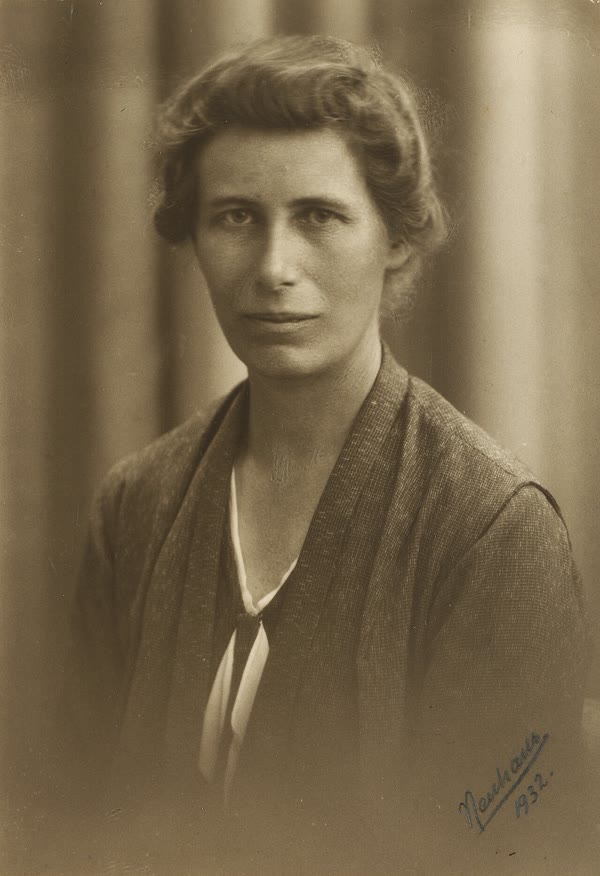
\includegraphics[width=\linewidth]{images/book3/b1-lehmann.jpg}

{\scriptsize Inge Lehmann en 1932, par Even Neuhaus. Domaine public.}
\end{minipage}
\end{history}

\section{Masse volumique, pesanteur et pression d'après les données sismiques}

Les vitesses sismiques donnent deux combinaisons des modules et de la masse
volumique, non la masse volumique elle-même. Une troisième relation vient de
l'hypothèse que, à l'intérieur d'une couche de composition uniforme, la roche est
simplement comprimée par le poids de la roche située au-dessus.

\begin{definition}[Paramètre sismique]\label{def:b1:layered-earth:seismic-parameter}
Le \emph{paramètre sismique}\index{parametre sismique@paramètre sismique} à une profondeur est
\[
  \Phi = v_P^2 - \tfrac43 v_S^2 = \frac{K}{\rho},
\]
le module d'incompressibilité divisé par la masse volumique, calculé à partir des
deux seules vitesses sismiques (\cref{prop:b1:layered-earth:speeds}).
\end{definition}

\begin{theorem}[Équation d'Adams--Williamson]\label{thm:b1:layered-earth:adams-williamson}
Dans une région de composition uniforme, en équilibre hydrostatique, comprimée de
façon adiabatique, la masse volumique varie avec le rayon selon
\[
  \frac{\mathrm d\rho}{\mathrm dr} = -\frac{\rho(r)\,g(r)}{\Phi(r)},
\]
où $g(r)$ est la pesanteur au rayon $r$.
\end{theorem}

\begin{proof}
L'équilibre hydrostatique donne $\mathrm dP/\mathrm dr = -\rho g$ (le rappel,
avec $\mathrm dz = -\mathrm dr$). Le module d'incompressibilité est défini par
$K = \rho\,\mathrm dP/\mathrm d\rho$ pour la compression considérée~; pour une
roche de composition fixe comprimée sans échange de chaleur, c'est le module
adiabatique que mesurent les ondes sismiques, donc
$\mathrm d\rho/\mathrm dP = \rho/K$.
Par la règle de dérivation en chaîne,
\[
  \frac{\mathrm d\rho}{\mathrm dr} = \frac{\mathrm d\rho}{\mathrm dP}\,
  \frac{\mathrm dP}{\mathrm dr} = \frac{\rho}{K}\,(-\rho g) = -\frac{\rho g}{K/\rho}
  = -\frac{\rho g}{\Phi}. \qedhere
\]
\end{proof}

L'équation tombe en défaut à une discontinuité, où la composition ou la structure
cristalline change, et partout où la température s'écarte de l'adiabate~; mais
entre les discontinuités elle rend très bien compte de l'augmentation observée de
la masse volumique avec la profondeur (panneau (c) de la figure ci-dessous).
Partir d'une masse volumique au sommet de chaque région, l'intégrer vers le bas,
et ajuster les valeurs de départ jusqu'à ce que la masse et le moment d'inertie
sortent justes, c'est ainsi que furent construits les premiers modèles de masse
volumique. Les deux nombres globaux sont des intégrales de la masse volumique.

\begin{proposition}[Masse, pesanteur, pression et moment d'inertie]
\label{prop:b1:layered-earth:integrals}
Pour une Terre à symétrie sphérique de rayon $R$ et de masse volumique $\rho(r)$,
la masse à l'intérieur du rayon $r$, la pesanteur, la pression et le moment
d'inertie par rapport à un axe passant par le centre sont
\[
  m(r) = \int_0^r 4\pi s^2\rho(s)\,\mathrm ds, \quad
  g(r) = \frac{G\,m(r)}{r^2}, \quad
  P(r) = \int_r^R \rho(s)\,g(s)\,\mathrm ds, \quad
  I = \frac{8\pi}{3}\int_0^R \rho(r)\,r^4\,\mathrm dr.
\]
\end{proposition}

\begin{proof}
Une mince coquille de rayon $s$ et d'épaisseur $\mathrm ds$ a pour volume
$4\pi s^2\,\mathrm ds$, d'où la première intégrale. La pesanteur d'un corps à
symétrie sphérique au-delà d'un rayon est celle de sa masse intérieure,
concentrée au centre, et les coquilles extérieures à $r$ attirent sans force
résultante (le théorème des coquilles, admis des livres de physique)~; d'où
$g(r)$. L'intégration de l'équation hydrostatique à partir de la surface, où
$P = 0$, donne $P(r)$. Pour le moment d'inertie, une mince coquille sphérique de
masse $\mathrm dm$ et de rayon $r$ a, par rapport aux trois axes $x$, $y$, $z$,
des moments dont la somme est
$\int (y^2 + z^2) + (z^2 + x^2) + (x^2 + y^2)\,\mathrm dm = 2r^2\,\mathrm dm$~;
par symétrie les trois sont égaux, donc chacun vaut $\tfrac23 r^2\,\mathrm dm$.
Avec $\mathrm dm = 4\pi r^2\rho\,\mathrm dr$, la sommation des coquilles donne $I$.
\end{proof}

Pour une sphère de masse volumique uniforme, $I = \tfrac{8\pi}{15}\rho R^5 = 0.4\,MR^2$.
Le facteur de la Terre $I/MR^2 = 0.3308$ est plus petit~: sa masse est concentrée
vers le centre, ce qui est le premier argument en faveur d'un noyau dense.
Calculées à partir de la seule masse volumique de PREM, les intégrales donnent une
masse de \qty{5.976e24}{kg} (\qty{0.06}{\percent} au-dessus de la valeur mesurée
\qty{5.972e24}{kg}), un facteur $0.3309$, et une pression centrale de
\qty{364}{GPa}, la valeur tabulée avec PREM à \qty{0.1}{\percent} près.

\begin{omfigure}
\begin{tabular}{@{}c@{\hspace{2mm}}c@{\hspace{2mm}}c@{}}
\begin{tikzpicture}
\begin{axis}[omrecord, omdepth, width=0.35\linewidth, height=7.0cm, xmin=0, xmax=12, ymin=0, ymax=6371,
  xlabel={$g$ (\unit{m.s^{-2}})}, ylabel={profondeur (km)}, ytick={0,1000,...,6000}, xtick={0,4,8,12},
  tick label style={font=\scriptsize}, label style={font=\small}]
\addplot[very thick, blue!70!black] table[x=g, y=depth] {figdata/out/bachelor-1-prem_profiles-functionals.dat};
\draw[black!35] (axis cs:0,2891) -- (axis cs:12,2891);
\draw[black!35] (axis cs:0,5149.5) -- (axis cs:12,5149.5);
\node[font=\scriptsize, anchor=south west] at (axis cs:0.3,2891) {CMB};
\node[font=\scriptsize, anchor=south west] at (axis cs:0.3,5149.5) {ICB};
\end{axis}
\end{tikzpicture}
&
\begin{tikzpicture}
\begin{axis}[omrecord, omdepth, width=0.35\linewidth, height=7.0cm, xmin=0, xmax=400, ymin=0, ymax=6371,
  xlabel={$P$ (GPa)}, ytick={0,1000,...,6000}, yticklabels={}, xtick={0,200,400},
  tick label style={font=\scriptsize}, label style={font=\small}]
\addplot[very thick, red!75!black] table[x=P, y=depth] {figdata/out/bachelor-1-prem_profiles-functionals.dat};
\draw[black!35] (axis cs:0,2891) -- (axis cs:400,2891);
\draw[black!35] (axis cs:0,5149.5) -- (axis cs:400,5149.5);
\node[font=\scriptsize, anchor=south west] at (axis cs:150,2891) {\qty{136}{GPa}};
\node[font=\scriptsize, anchor=south east] at (axis cs:290,5149.5) {\qty{329}{GPa}};
\end{axis}
\end{tikzpicture}
&
\begin{tikzpicture}
\begin{axis}[omrecord, omdepth, width=0.35\linewidth, height=7.0cm, xmin=2, xmax=14, ymin=0, ymax=6371,
  xlabel={$\rho$ (\unit{g.cm^{-3}})}, ytick={0,1000,...,6000}, yticklabels={}, xtick={2,6,10,14},
  tick label style={font=\scriptsize}, label style={font=\small},
  legend style={font=\scriptsize, at={(0.97,0.97)}, anchor=north east, draw=none, fill=white}]
\addplot[very thick, black!55] table[x=rho, y=depth] {figdata/out/bachelor-1-prem_profiles-profiles.dat};
\addlegendentry{PREM}
\addplot[only marks, mark=o, mark size=1.4pt, orange!85!black, each nth point=15, unbounded coords=discard]
  table[x=rho_aw, y=depth] {figdata/out/bachelor-1-prem_profiles-adams.dat};
\addlegendentry{Adams--Williamson}
\end{axis}
\end{tikzpicture}
\\[2pt]
{\small (a) pesanteur} & {\small (b) pression} & {\small (c) autocompression}
\end{tabular}

\par\smallskip{\small À l'intérieur de la Terre, d'après PREM. (a) et (b) Pesanteur
et pression calculées à partir de la masse volumique de PREM avec la
\cref{prop:b1:layered-earth:integrals}~: la pesanteur reste voisine de
\qty{10}{m.s^{-2}} dans le \omterm{def:b1:layered-earth:layers}{manteau}, culmine à \qty{10.7}{m.s^{-2}} à la \omterm{def:b1:layered-earth:discontinuity}{limite
noyau--manteau} (CMB) et tombe à zéro au centre~; la pression atteint \qty{136}{GPa}
à la CMB, \qty{329}{GPa} à la \omterm{def:b1:layered-earth:discontinuity}{limite du noyau interne} (ICB) et \qty{364}{GPa} au
centre. (c) L'équation d'Adams--Williamson, intégrée vers le bas à partir de la
masse volumique de PREM à \qty{771}{km} et au sommet du \omterm{def:b1:layered-earth:layers}{noyau externe} avec les
vitesses et la pesanteur de PREM (cercles), suit PREM à \qty{0.2}{\percent} près~:
là, l'augmentation de la masse volumique est la compression d'un matériau
uniforme~; les sauts ne le sont pas.}
\end{omfigure}

Que la pesanteur croisse en descendant dans le \omterm{def:b1:layered-earth:layers}{manteau} est une conséquence directe
du noyau dense~: la masse qui reste à l'intérieur du rayon diminue plus lentement
que $r^2$. À travers le \omterm{def:b1:layered-earth:layers}{manteau} $g$ ne change guère, et la pression croît presque
linéairement avec la profondeur, d'environ \qty{4.7}{GPa} par cent kilomètres.


\section{Le manteau~: une roche, plusieurs assemblages minéralogiques}

Le \omterm{def:b1:layered-earth:layers}{manteau} supérieur est de la péridotite, connue par les fragments que les
volcans ramènent et par des tranches de \omterm{def:b1:layered-earth:layers}{manteau} charriées sur les continents~:
d'environ la moitié aux trois cinquièmes d'\omterm{def:b1:rock-forming-minerals:groups}{olivine} en volume
(\qtyrange{49}{62}{\percent} dans les compositions proposées), le reste de
\omterm{def:b1:rock-forming-minerals:groups}{pyroxènes} et d'un \omterm{def:b1:rock-forming-minerals:mineral}{minéral} alumineux (\omterm{def:b1:rock-forming-minerals:groups}{plagioclase}, spinelle ou \omterm{def:b1:rock-forming-minerals:groups}{grenat}, selon la
profondeur). La pression qui croît avec la profondeur ne change pas cette
composition, mais contraint ses atomes à des arrangements plus denses~: des
\omterm{def:b1:rock-forming-minerals:polymorph}{polymorphes} (\cref{ch:b1:rock-forming-minerals}) apparaissent les uns après les
autres.

\begin{definition}[Zone de transition du manteau]\label{def:b1:layered-earth:transition-zone}
La \emph{zone de transition du manteau}\index{zone de transition du manteau} est la partie
du \omterm{def:b1:layered-earth:layers}{manteau} comprise entre les \omterm{def:b1:layered-earth:discontinuity}{discontinuités sismiques} voisines de \qty{410}{km} et
\qty{660}{km} de profondeur, dans laquelle l'\omterm{def:b1:rock-forming-minerals:groups}{olivine} du \omterm{def:b1:layered-earth:layers}{manteau} supérieur est
remplacée par ses \omterm{def:b1:rock-forming-minerals:polymorph}{polymorphes} plus denses, la wadsleyite puis la ringwoodite.
Au-dessus se trouve le \omterm{def:b1:layered-earth:layers}{manteau} supérieur~; au-dessous, le \omterm{def:b1:layered-earth:layers}{manteau} inférieur,
jusqu'à la \omterm{def:b1:layered-earth:discontinuity}{limite noyau--manteau}.
\end{definition}

Vers \qty{410}{km} (\qty{14}{GPa}), l'\omterm{def:b1:rock-forming-minerals:groups}{olivine} \ce{(Mg,Fe)2SiO4} devient
wadsleyite, de même formule~; vers \qty{520}{km} (\qty{17.5}{GPa}), la wadsleyite
devient ringwoodite~; les \omterm{def:b1:rock-forming-minerals:groups}{pyroxènes} se dissolvent dans un \omterm{def:b1:rock-forming-minerals:groups}{grenat} riche en silicium,
la majorite, si bien qu'au milieu de la zone de transition le \omterm{def:b1:rock-forming-minerals:groups}{grenat} les contient
tous, et que la zone est un peu plus qu'à moitié faite de \omterm{def:b1:rock-forming-minerals:polymorph}{polymorphes} de l'\omterm{def:b1:rock-forming-minerals:groups}{olivine},
le reste étant du \omterm{def:b1:rock-forming-minerals:groups}{grenat}. Vers \qty{660}{km}, à une pression voisine de
\qty{24}{GPa}, la ringwoodite se décompose en
deux minéraux, écrits pour le pôle magnésien
\[
  \ce{Mg2SiO4 -> MgSiO3 + MgO}:
\]
bridgmanite, \ce{(Mg,Fe)SiO3} de structure pérovskite, et ferropériclase,
\ce{(Mg,Fe)O}. Un \omterm{def:b1:layered-earth:layers}{manteau} inférieur de même composition que le \omterm{def:b1:layered-earth:layers}{manteau} supérieur
est constitué d'environ \qty{75}{\percent} de bridgmanite, \qty{17}{\percent} de
ferropériclase et \qty{8}{\percent} d'une pérovskite calcique en volume, et
s'accorde avec les masses volumiques et les vitesses du modèle de référence. La
bridgmanite est donc le \omterm{def:b1:rock-forming-minerals:mineral}{minéral} le plus abondant de la Terre~; elle n'a reçu son
nom qu'en 2014, après la description de grains naturels dans une météorite
fortement choquée.
% ledger: frost:mantle-transitions, sun:lower-mantle, tschauner:bridgmanite

Chaque changement produit des minéraux plus denses, donc il élève la masse
volumique et les vitesses sismiques~: les transitions sont les discontinuités des
profils (figure ci-dessous). Leurs
profondeurs ne sont pas fixes. Un changement de phase se produit à une pression
qui dépend de la température, et la pente de cette dépendance (la pente de
Clapeyron, traitée dans le volume de deuxième année) fait remonter la
discontinuité de \qty{410}{km} et descendre celle de \qty{660}{km} dans la roche
froide d'un panneau plongeant. Cartographier la topographie des discontinuités
est l'une des façons de repérer les régions froides et chaudes du \omterm{def:b1:layered-earth:layers}{manteau}.

\begin{omfigure}
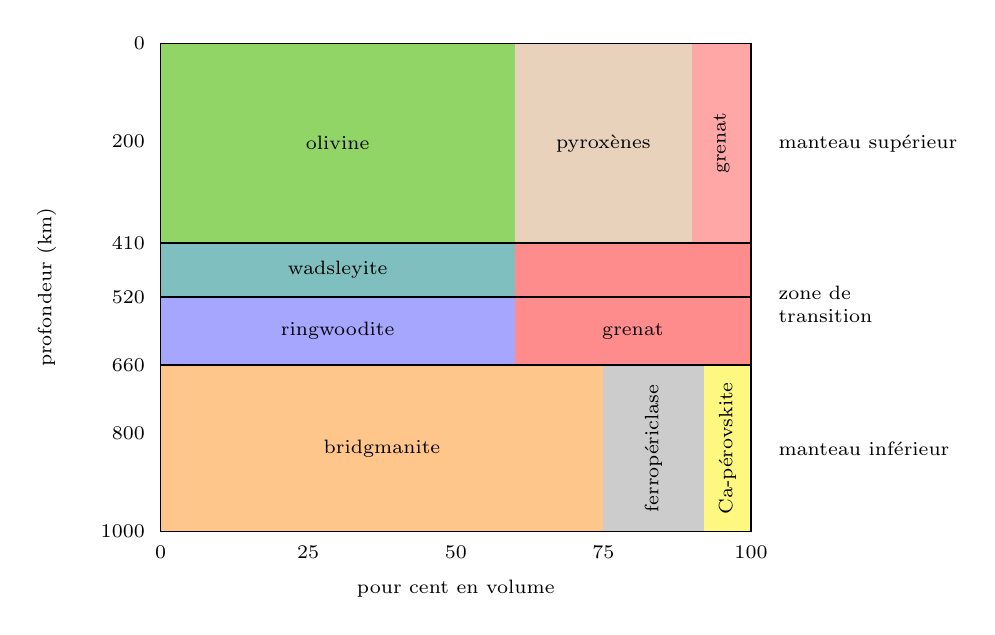
\begin{tikzpicture}[x=0.075mm, y=-0.062mm, font=\scriptsize]
% schematic volume fractions (ledger frost:mantle-transitions, sun:lower-mantle)
\def\W{1000}
% upper mantle 0-410: olivine 60, pyroxenes 30, garnet 10
\fill[green!45!olive!60] (0,0) rectangle (600,410);
\fill[brown!35] (600,0) rectangle (900,410);
\fill[red!35] (900,0) rectangle (1000,410);
% 410-520 wadsleyite 60, garnet 40 ; 520-660 ringwoodite 60, garnet 40
\fill[teal!50] (0,410) rectangle (600,520);
\fill[blue!35] (0,520) rectangle (600,660);
\fill[red!45] (600,410) rectangle (1000,660);
% 660-1000 bridgmanite 75, ferropericlase 17, Ca-perovskite 8
\fill[orange!45] (0,660) rectangle (750,1000);
\fill[gray!40] (750,660) rectangle (920,1000);
\fill[yellow!50] (920,660) rectangle (1000,1000);
\draw (0,0) rectangle (1000,1000);
\foreach \d in {410,520,660} \draw[thick] (0,\d) -- (1000,\d);
\node at (300,205) {olivine};
\node[align=center] at (750,205) {pyroxènes};
\node[rotate=90] at (950,205) {grenat};
\node at (300,465) {wadsleyite};
\node at (300,590) {ringwoodite};
\node[align=center] at (800,590) {grenat};
\node at (375,830) {bridgmanite};
\node[rotate=90, align=center] at (835,830) {ferropériclase};
\node[rotate=90] at (960,830) {Ca-pérovskite};
\foreach \d in {0,200,410,520,660,800,1000} \node[anchor=east] at (-10,\d) {\d};
\node[rotate=90, anchor=south] at (-160,500) {profondeur (km)};
\foreach \p in {0,25,50,75,100} \node[anchor=north] at (\p*10,1010) {\p};
\node[anchor=north] at (500,1080) {pour cent en volume};
\node[anchor=west, align=left] at (1030,205) {manteau supérieur};
\node[anchor=west, align=left] at (1030,535) {zone de\\transition};
\node[anchor=west, align=left] at (1030,830) {manteau inférieur};
\end{tikzpicture}

\par\smallskip{\small Les minéraux d'un \omterm{def:b1:layered-earth:layers}{manteau} de péridotite en fonction de la
profondeur, en fractions volumiques (schématique~: les limites sont dessinées
nettes, et les fractions sont des valeurs rondes dans les intervalles cités dans
le texte). La composition ne change pas~; les minéraux, si, vers 410, 520 et
\qty{660}{km}.}
\end{omfigure}

À la base du \omterm{def:b1:layered-earth:layers}{manteau}, la couche appelée D$''$ (D seconde, nom conservé d'un des
premiers modèles de la Terre) a un gradient de vitesse différent du reste du
\omterm{def:b1:layered-earth:layers}{manteau} inférieur~; PREM lui attribue les \qty{150}{km} les plus bas du \omterm{def:b1:layered-earth:layers}{manteau}.
Elle est hétérogène du point de vue sismique~: plages de très faible vitesse,
forts gradients, réflecteurs. On pense que c'est une couche limite entre le noyau
chaud et le \omterm{def:b1:layered-earth:layers}{manteau}, et peut-être un cimetière de vieux panneaux plongeants.
% ledger: prem:dpp

\section{Le noyau}

Le noyau est surtout du fer. Sa masse volumique, ses vitesses et son aptitude à
engendrer un champ magnétique indiquent tous un métal, et le fer est de loin
l'élément le plus abondant qui soit assez dense parmi ceux que les météorites et
le Soleil montrent être courants. Le nickel, abondant dans les météorites de fer,
l'accompagne. Mais le noyau n'est pas du fer--nickel pur.
\begin{itemize}
  \item Le noyau est de \qtyrange{5}{10}{\percent} moins dense que ne le serait du
        fer pur à la même pression et à la même température~: il doit contenir
        des éléments légers, parmi lesquels le silicium, le soufre, le carbone,
        l'oxygène et l'hydrogène sont les candidats.
  \item La masse volumique saute d'environ \qty{4.5}{\percent} à la \omterm{def:b1:layered-earth:discontinuity}{limite du
        noyau interne}, trop pour la congélation d'un seul et même métal~: le
        \omterm{def:b1:layered-earth:layers}{noyau interne} contient lui aussi des éléments légers, mais moins, quelques
        pour cent contre \qtyrange{5}{10}{\percent} dans le liquide.
\end{itemize}
% ledger: badro:core
La différence a une conséquence. À mesure que la Terre se refroidit --- son \omterm{def:b1:layered-earth:layers}{manteau}
d'environ \qty{100}{\degreeCelsius} par milliard d'années actuellement --- le
liquide du noyau gèle sur le \omterm{def:b1:layered-earth:layers}{noyau interne}, qui croît, et
% ledger: bellini:cooling
la congélation laisse la plupart des éléments légers dans le liquide. Le liquide
léger libéré à la base du \omterm{def:b1:layered-earth:layers}{noyau externe} remonte, et l'on pense que cette
flottabilité contribue à brasser le \omterm{def:b1:layered-earth:layers}{noyau externe} et à entretenir la dynamo qui
produit le champ magnétique de la Terre.

\section{Couches mécaniques~: lithosphère et asthénosphère}

Les couches ci-dessus sont définies par la composition et la phase~: la \omterm{def:b1:layered-earth:layers}{croûte} et
le \omterm{def:b1:layered-earth:layers}{manteau} sont des roches différentes, le \omterm{def:b1:layered-earth:layers}{noyau externe} et le \omterm{def:b1:layered-earth:layers}{noyau interne} des
états différents. La tectonique des plaques demande une autre division, selon la
résistance, qui recoupe la première.

\begin{definition}[Lithosphère, asthénosphère, zone à faible vitesse]
\label{def:b1:layered-earth:lithosphere}
La \emph{lithosphère}\index{lithosphere@lithosphère} est l'enveloppe rigide externe de la
Terre, la \omterm{def:b1:layered-earth:layers}{croûte} et le \omterm{def:b1:layered-earth:layers}{manteau} le plus supérieur, qui se comporte comme une couche
résistante sur les durées géologiques et est divisée en plaques.
L'\emph{asthénosphère}\index{asthenosphere@asthénosphère} est la couche plus faible du \omterm{def:b1:layered-earth:layers}{manteau} supérieur située
au-dessous, qui se déforme par écoulement lent et laisse les plaques se déplacer.
La \emph{zone à faible vitesse}\index{zone a faible vitesse@zone à faible vitesse} est l'intervalle de profondeur sous la lithosphère où
les vitesses sismiques, surtout celles des ondes S, sont plus faibles
qu'immédiatement au-dessus et au-dessous.
\end{definition}

La \omterm{def:b1:layered-earth:lithosphere}{lithosphère} n'est pas une roche mais un intervalle de température~: la
péridotite du \omterm{def:b1:layered-earth:layers}{manteau} est résistante là où elle est froide et flue là où elle est
chaude, et sa base est à peu près une isotherme. Elle est mince sous les dorsales,
où le \omterm{def:b1:layered-earth:layers}{manteau} chaud monte, d'environ \qty{140}{km} d'épaisseur sous le plus vieux
fond océanique, et de \qtyrange{40}{280}{km} sous les continents, la plus épaisse
sous les vieux cratons~; le sommet de l'\omterm{def:b1:layered-earth:lithosphere}{asthénosphère} se trouve à environ
\qtyrange{80}{200}{km}. Du point de vue sismique, l'\omterm{def:b1:layered-earth:lithosphere}{asthénosphère} se manifeste
comme la \omterm{def:b1:layered-earth:lithosphere}{zone à faible vitesse}, proche de ses conditions de fusion~: dans PREM, la
vitesse S diminue légèrement depuis le \omterm{def:b1:layered-earth:discontinuity}{Moho} jusqu'à \qty{220}{km}, où elle remonte
d'un saut. La façon dont la résistance dépend de la température, et pourquoi, fait
l'objet du \cref{ch:b1:stress-strain-rheology}.

\begin{inthefield}[Une station sismique]
\begin{minipage}[t]{0.55\linewidth}\vspace{0pt}
Les temps de trajet sur lesquels reposent les modèles de référence viennent de
stations permanentes. Un sismomètre large bande, qui enregistre les mouvements du
sol sur des périodes allant du centième de seconde à des heures, repose sur un
pilier de béton posé sur la roche nue et isolé du sol de la chambre, sous un
couvercle qui garde sa température stable~: une variation d'une fraction de
degré, un courant d'air ou le passage d'un camion se verrait sur l'enregistrement.
L'enregistreur date chaque échantillon avec l'heure fournie par des satellites, et
les enregistrements sont transmis en continu à des centres de données qui les
partagent librement. Des réseaux de telles stations localisent et datent chaque
grand séisme~; les temps d'arrivée pointés sur leurs enregistrements ont été
inversés pour obtenir les vitesses à chaque profondeur.
\end{minipage}\hfill
\begin{minipage}[t]{0.42\linewidth}\vspace{0pt}
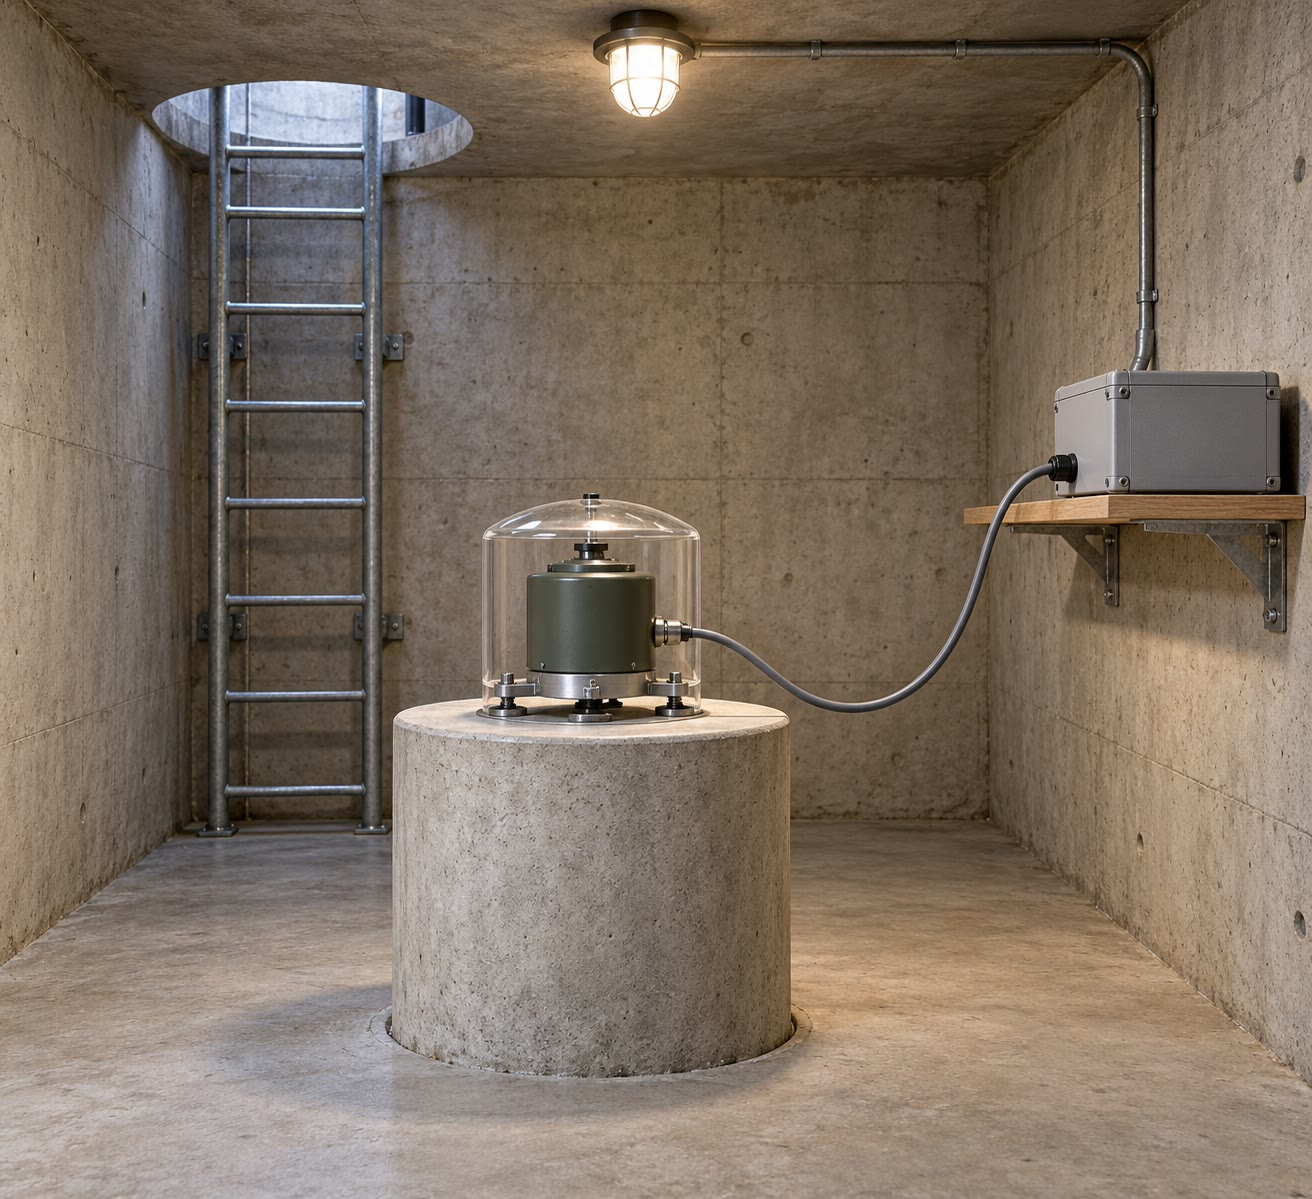
\includegraphics[width=\linewidth]{images/book3/ai/b1-seismometer-vault.jpg}

{\scriptsize Un sismomètre large bande sur son pilier dans une chambre
souterraine, avec l'enregistreur sur le mur (illustration générée par IA).}
\end{minipage}
\end{inthefield}

\section{Exercices}

\begin{exercise}[$\star$]\label{exo:b1:layered-earth:1}
Avec les rayons de PREM $R = \qty{6371}{km}$, $r_{\text{CMB}} = \qty{3480}{km}$ et
$r_{\text{ICB}} = \qty{1221.5}{km}$, calculer les fractions du volume de la Terre
occupées par le noyau et par le \omterm{def:b1:layered-earth:layers}{noyau interne}.
% ledger: prem:cmb, prem:icb
\end{exercise}

\begin{exercise}[$\star$]\label{exo:b1:layered-earth:2}
Juste au-dessus de la \omterm{def:b1:layered-earth:discontinuity}{limite noyau--manteau}, PREM donne $v_P = \qty{13.7166}{km.s^{-1}}$,
$v_S = \qty{7.26466}{km.s^{-1}}$, $\rho = \qty{5.56645}{g.cm^{-3}}$~; juste au-dessous,
$v_P = \qty{8.06482}{km.s^{-1}}$, $v_S = 0$, $\rho = \qty{9.90349}{g.cm^{-3}}$.
Calculer le \omterm{def:b1:layered-earth:seismic-parameter}{paramètre sismique} et le module d'incompressibilité de chaque côté (en
GPa). Qu'est-ce qui change le plus à travers la limite~?
% ledger: data:prem, prem:cmb
\end{exercise}

\begin{exercise}[$\star$]\label{exo:b1:layered-earth:3}
Une \omterm{def:b1:layered-earth:layers}{croûte} de \qty{30}{km} d'épaisseur, à \qty{6.2}{km.s^{-1}}, repose sur un
\omterm{def:b1:layered-earth:layers}{manteau} à \qty{8.1}{km.s^{-1}}. Calculer l'angle critique, la distance critique et
la \omterm{def:b1:layered-earth:head-wave}{distance de croisement}.
\end{exercise}

\begin{exercise}[$\star$]\label{exo:b1:layered-earth:4}
La masse du noyau est de \qty{1.94e24}{kg} et son rayon de \qty{3480}{km}.
Calculer la pesanteur à la \omterm{def:b1:layered-earth:discontinuity}{limite noyau--manteau} et la comparer à la pesanteur de
surface, \qty{9.82}{m.s^{-2}}. Pourquoi est-elle plus grande~?
\end{exercise}

\begin{exercise}[$\star\star$]\label{exo:b1:layered-earth:5}
Sur un profil de réfraction, les premières arrivées sont à \qty{10.0}{s} pour
\qty{60}{km}, à \qty{33.3}{s} pour \qty{200}{km} et à \qty{45.8}{s} pour
\qty{300}{km}~; la droite passant par le premier point passe par l'origine.
Trouver $v_1$, $v_2$, le temps d'interception et la profondeur de la limite, et
vérifier le résultat avec la \omterm{def:b1:layered-earth:head-wave}{distance de croisement}.
\end{exercise}

\begin{exercise}[$\star\star$]\label{exo:b1:layered-earth:6}
Montrer qu'une sphère homogène a $I = 0.4\,MR^2$. Calculer ensuite la masse et le
facteur $I/MR^2$ d'une Terre à deux couches~: un noyau de rayon \qty{3480}{km} et
de masse volumique \qty{11.0}{g.cm^{-3}} dans un \omterm{def:b1:layered-earth:layers}{manteau} de masse volumique
\qty{4.45}{g.cm^{-3}}, avec $R = \qty{6371}{km}$. Comparer à \num{5.972e24} kg et
$0.3308$.
\end{exercise}

\begin{exercise}[$\star\star$]\label{exo:b1:layered-earth:7}
À \qty{1471}{km} de profondeur, PREM donne $v_P = \qty{12.16}{km.s^{-1}}$,
$v_S = \qty{6.673}{km.s^{-1}}$, $\rho = \qty{4.86}{g.cm^{-3}}$, et la pesanteur
est de \qty{9.9}{m.s^{-2}}. Calculer le gradient de masse volumique donné par
l'équation d'Adams--Williamson, en \unit{g.cm^{-3}} par \qty{1000}{km}, et le
comparer aux masses volumiques de PREM, \num{4.844} à \qty{1471}{km} et
\num{5.357} à \qty{2471}{km}.
% ledger: data:prem
\end{exercise}

\begin{exercise}[$\star\star$]\label{exo:b1:layered-earth:8}
Estimer la pression à \qty{670}{km} de profondeur à partir d'une masse volumique
moyenne de \qty{3.57}{g.cm^{-3}} et d'une pesanteur de \qty{9.9}{m.s^{-2}}. Quel
changement minéralogique y est attendu~?
% ledger: frost:mantle-transitions
\end{exercise}

\begin{exercise}[$\star\star$]\label{exo:b1:layered-earth:9}
La masse volumique moyenne du \omterm{def:b1:layered-earth:layers}{noyau externe} dans PREM est de
\qty{10.90}{g.cm^{-3}}~; à la \omterm{def:b1:layered-earth:discontinuity}{limite du noyau interne}, sa masse volumique est de
\qty{12.166}{g.cm^{-3}} au-dessus et de \qty{12.764}{g.cm^{-3}} au-dessous.
(a)~Si le fer dans les mêmes conditions est de \qtyrange{5}{10}{\percent} plus
dense que le \omterm{def:b1:layered-earth:layers}{noyau externe}, quel intervalle de masses volumiques cela donne-t-il
pour le fer liquide à cet endroit~? (b)~Calculer le saut de masse volumique à la
\omterm{def:b1:layered-earth:discontinuity}{limite du noyau interne} en pour cent, et le comparer aux \qty{4.5}{\percent} des
études récentes. (c)~Que dit, sur les éléments légers, un saut plus grand que ce
que donnerait la congélation seule~?
% ledger: badro:core, prem:icb
\end{exercise}

\begin{exercise}[$\star\star\star$]\label{exo:b1:layered-earth:10}
Montrer que le temps de l'onde réfléchie $t_r(x) = \sqrt{x^2 + 4h^2}/v_1$ et le
temps de l'\omterm{def:b1:layered-earth:head-wave}{onde conique} du \cref{thm:b1:layered-earth:two-layer} sont égaux, et
ont des pentes égales, en $x = 2h\tan i_c$, et que $t_r > t_{\text{conique}}$
au-delà. Interpréter.
\end{exercise}

\begin{exercise}[$\star\star\star$]\label{exo:b1:layered-earth:11}
Pour une Terre de masse volumique uniforme $\rho$, montrer que
$g(r) = \tfrac43\pi G\rho r$ et $P(r) = \tfrac23\pi G\rho^2(R^2 - r^2)$. Calculer la
pression centrale avec $\rho = \qty{5513}{kg.m^{-3}}$ et $R = \qty{6371}{km}$, et la
comparer à la valeur de PREM, \qty{363.85}{GPa}.
% ledger: earth:density, prem:centre
\end{exercise}

\begin{exercise}[$\star\star\star$]\label{exo:b1:layered-earth:12}
Montrer que si $g/\Phi$ est constant dans une couche, l'équation d'Adams--Williamson
donne $\rho = \rho_0\exp\bigl(g(z - z_0)/\Phi\bigr)$ avec la profondeur $z$.
L'appliquer au \omterm{def:b1:layered-earth:layers}{noyau externe}, de \qty{2891}{km} ($\rho_0 =
\qty{9.90}{g.cm^{-3}}$) à \qty{5149.5}{km}, avec les valeurs moyennes
$g = \qty{7.9}{m.s^{-2}}$ et $\Phi = \qty{87}{km^2.s^{-2}}$~; comparer à la valeur
de PREM, \qty{12.17}{g.cm^{-3}}, à la \omterm{def:b1:layered-earth:discontinuity}{limite du noyau interne}.
% ledger: prem:icb
\end{exercise}

\section{Problème~: Peser les enveloppes de la Terre}

\begin{problem}[{Problème du week-end --- volumes, masses et moment d'inertie d'une
Terre à quatre enveloppes construite à partir de PREM, comparés à la masse et au
moment d'inertie mesurés~; pesanteur et pression en profondeur}]
\label{pb:b1:layered-earth:1}
% values: calc/ch09.py; mean densities rounded from figdata prem_profiles (values part)
% ledger: data:prem, prem:constraints, prem:centre, prem:cmb, earth:mass, earth:MoI, const:G
La Terre est découpée en quatre enveloppes aux rayons de PREM, et chacune reçoit
sa masse volumique moyenne dans PREM, arrondie~:
\begin{center}
\small
\begin{tabular}{lccc}
\hline
enveloppe & de (km) & à (km) & masse vol. moyenne (\unit{g.cm^{-3}}) \\
\hline
\omterm{def:b1:layered-earth:layers}{croûte}, \omterm{def:b1:layered-earth:layers}{manteau} supérieur et zone de transition & 5701 & 6371 & 3.57 \\
\omterm{def:b1:layered-earth:layers}{manteau} inférieur & 3480 & 5701 & 4.90 \\
\omterm{def:b1:layered-earth:layers}{noyau externe} & 1221.5 & 3480 & 10.90 \\
\omterm{def:b1:layered-earth:layers}{noyau interne} & 0 & 1221.5 & 12.89 \\
\hline
\end{tabular}
\end{center}
On prend $G = \qty{6.674e-11}{m^3.kg^{-1}.s^{-2}}$. La masse mesurée de la Terre
est \qty{5.972e24}{kg} et son \omterm{def:b1:comparative-planetology:moi}{facteur de moment d'inertie} $I/MR^2 = 0.3308$.

\medskip
\noindent\textbf{Partie I --- Volumes.}
\begin{enumerate}
  \item Calculer le volume de la Terre.
  \item Calculer le volume de chaque enveloppe.
  \item Quelle fraction du volume chaque enveloppe occupe-t-elle~? Quelle
        enveloppe est la plus grande~?
  \item Quelle fraction du volume est du noyau~?
\end{enumerate}

\noindent\textbf{Partie II --- Masses.}
\begin{enumerate}[resume]
  \item Calculer la masse de chaque enveloppe.
  \item Les additionner, et comparer le total à la masse mesurée.
  \item En déduire la masse volumique moyenne de la Terre modèle.
  \item Quelle fraction de la masse est dans le \omterm{def:b1:layered-earth:layers}{noyau interne}~?
  \item Quelle fraction de la masse est dans le \omterm{def:b1:layered-earth:layers}{manteau} et la \omterm{def:b1:layered-earth:layers}{croûte} ensemble~?
  \item Comparer la part du noyau dans le volume et dans la masse, et expliquer.
\end{enumerate}

\noindent\textbf{Partie III --- Moment d'inertie.}
\begin{enumerate}[resume]
  \item Montrer, à partir de la \cref{prop:b1:layered-earth:integrals}, qu'une
        enveloppe uniforme comprise entre $r_1$ et $r_2$ a
        $I = \tfrac{8\pi}{15}\rho\,(r_2^5 - r_1^5)$.
  \item Calculer le moment d'inertie de chaque enveloppe.
  \item Quelle enveloppe contribue le plus, et pourquoi le \omterm{def:b1:layered-earth:layers}{noyau interne} ne
        contribue-t-il presque pas~?
  \item Les additionner et calculer $I/MR^2$ pour le modèle.
  \item Comparer à $0.3308$ et au $0.4$ d'une sphère homogène.
  \item Dans chaque enveloppe réelle, la masse volumique croît avec la profondeur.
        Cela explique-t-il que le facteur du modèle soit trop élevé~? Expliquer.
\end{enumerate}

\noindent\textbf{Partie IV --- Pesanteur et pression.}
\begin{enumerate}[resume]
  \item Calculer la pesanteur à la surface du modèle.
  \item Calculer la pesanteur à la \omterm{def:b1:layered-earth:discontinuity}{limite noyau--manteau}.
  \item Calculer la masse volumique moyenne du \omterm{def:b1:layered-earth:layers}{manteau} et de la \omterm{def:b1:layered-earth:layers}{croûte} ensemble.
  \item La pesanteur dans le \omterm{def:b1:layered-earth:layers}{manteau} reste voisine de \qty{10}{m.s^{-2}}. Estimer
        la pression à la \omterm{def:b1:layered-earth:discontinuity}{limite noyau--manteau}, et la comparer à la valeur de
        PREM, \qty{135.75}{GPa}.
  \item Calculer la masse volumique moyenne du noyau, et l'augmentation de
        pression de la \omterm{def:b1:layered-earth:discontinuity}{limite noyau--manteau} au centre dans un noyau uniforme,
        $\tfrac23\pi G\rho_c^2 r_c^2$ (\cref{exo:b1:layered-earth:11} appliqué au
        noyau seul).
  \item Les additionner pour estimer la pression centrale, et la comparer à la
        valeur de PREM, \qty{363.85}{GPa}. Pourquoi l'estimation est-elle trop
        basse~?
  \item Lesquels des nombres du modèle sont vérifiés par une mesure, et lesquels
        seulement par PREM lui-même~?
  \item Quelle fraction de la masse de la Terre se trouve dans le noyau~?
\end{enumerate}
\end{problem}
